\chapter{Methodology}

%TODO:Maybe cite example(s) of non-free-living data
\section{Datasets}
For our experiments we were interested in testing our algorithms on real-world free-living
data. In the past researchers have gathered activity data under unrealistic
laboratory conditions, and unfortunately there are not many labeled free-living
datasets publicly available. We tested our algorithms on two datasets that were
available to us. The first was synthetically generated by concatenating lab
visit data together, while the second was real-world free-living data.

\subsection{Synthetic Data (OSU Hip)}
We generated a synthetic, free-living dataset using physical activity data
collected by Stewart Trost of the Nutrition and Exercise Sciences department of
Oregon State University \cite{trost12}, \cite{zheng12}.
This dataset consisted of 91 time series collected over a 2-week period in a
laboratory environment, from 50 children between the ages of 5 and 15. Subjects
performed 12 different types of activities  over two separate lab visits, with
a hip-worn ActiGraph GT1M accelerometer that collected triaxial acceleration
data at a frequency of 30Hz (see top graph of Figure \ref{fig:timeseries}).

Data was collected from two separate visits to the lab, where the subjects performed 6 activities per visit.
Each subject performed the 12 activities in the same order.
In the version of the dataset available to us, we had all 12 activities of
41 of the subjects, only the first 6 activities of an additional 5 subjects,
and the last 6 activities of the remaining 4 subjects.
Subjects were given breaks in between each activity and activities lasted 5-10
minutes, however, these unlabelled breaks were removed from the version that we
used. Additionally, only two minutes of data were available for each subject, so 
time series consisted of six 120 second long activities. We concatenated the
data from these six activities together to create a synthetic, free-living dataset. 
Each of the 91 time series contained a total of $6*120*30 = 21600$ data ticks.

\begin{figure}
 \centering
 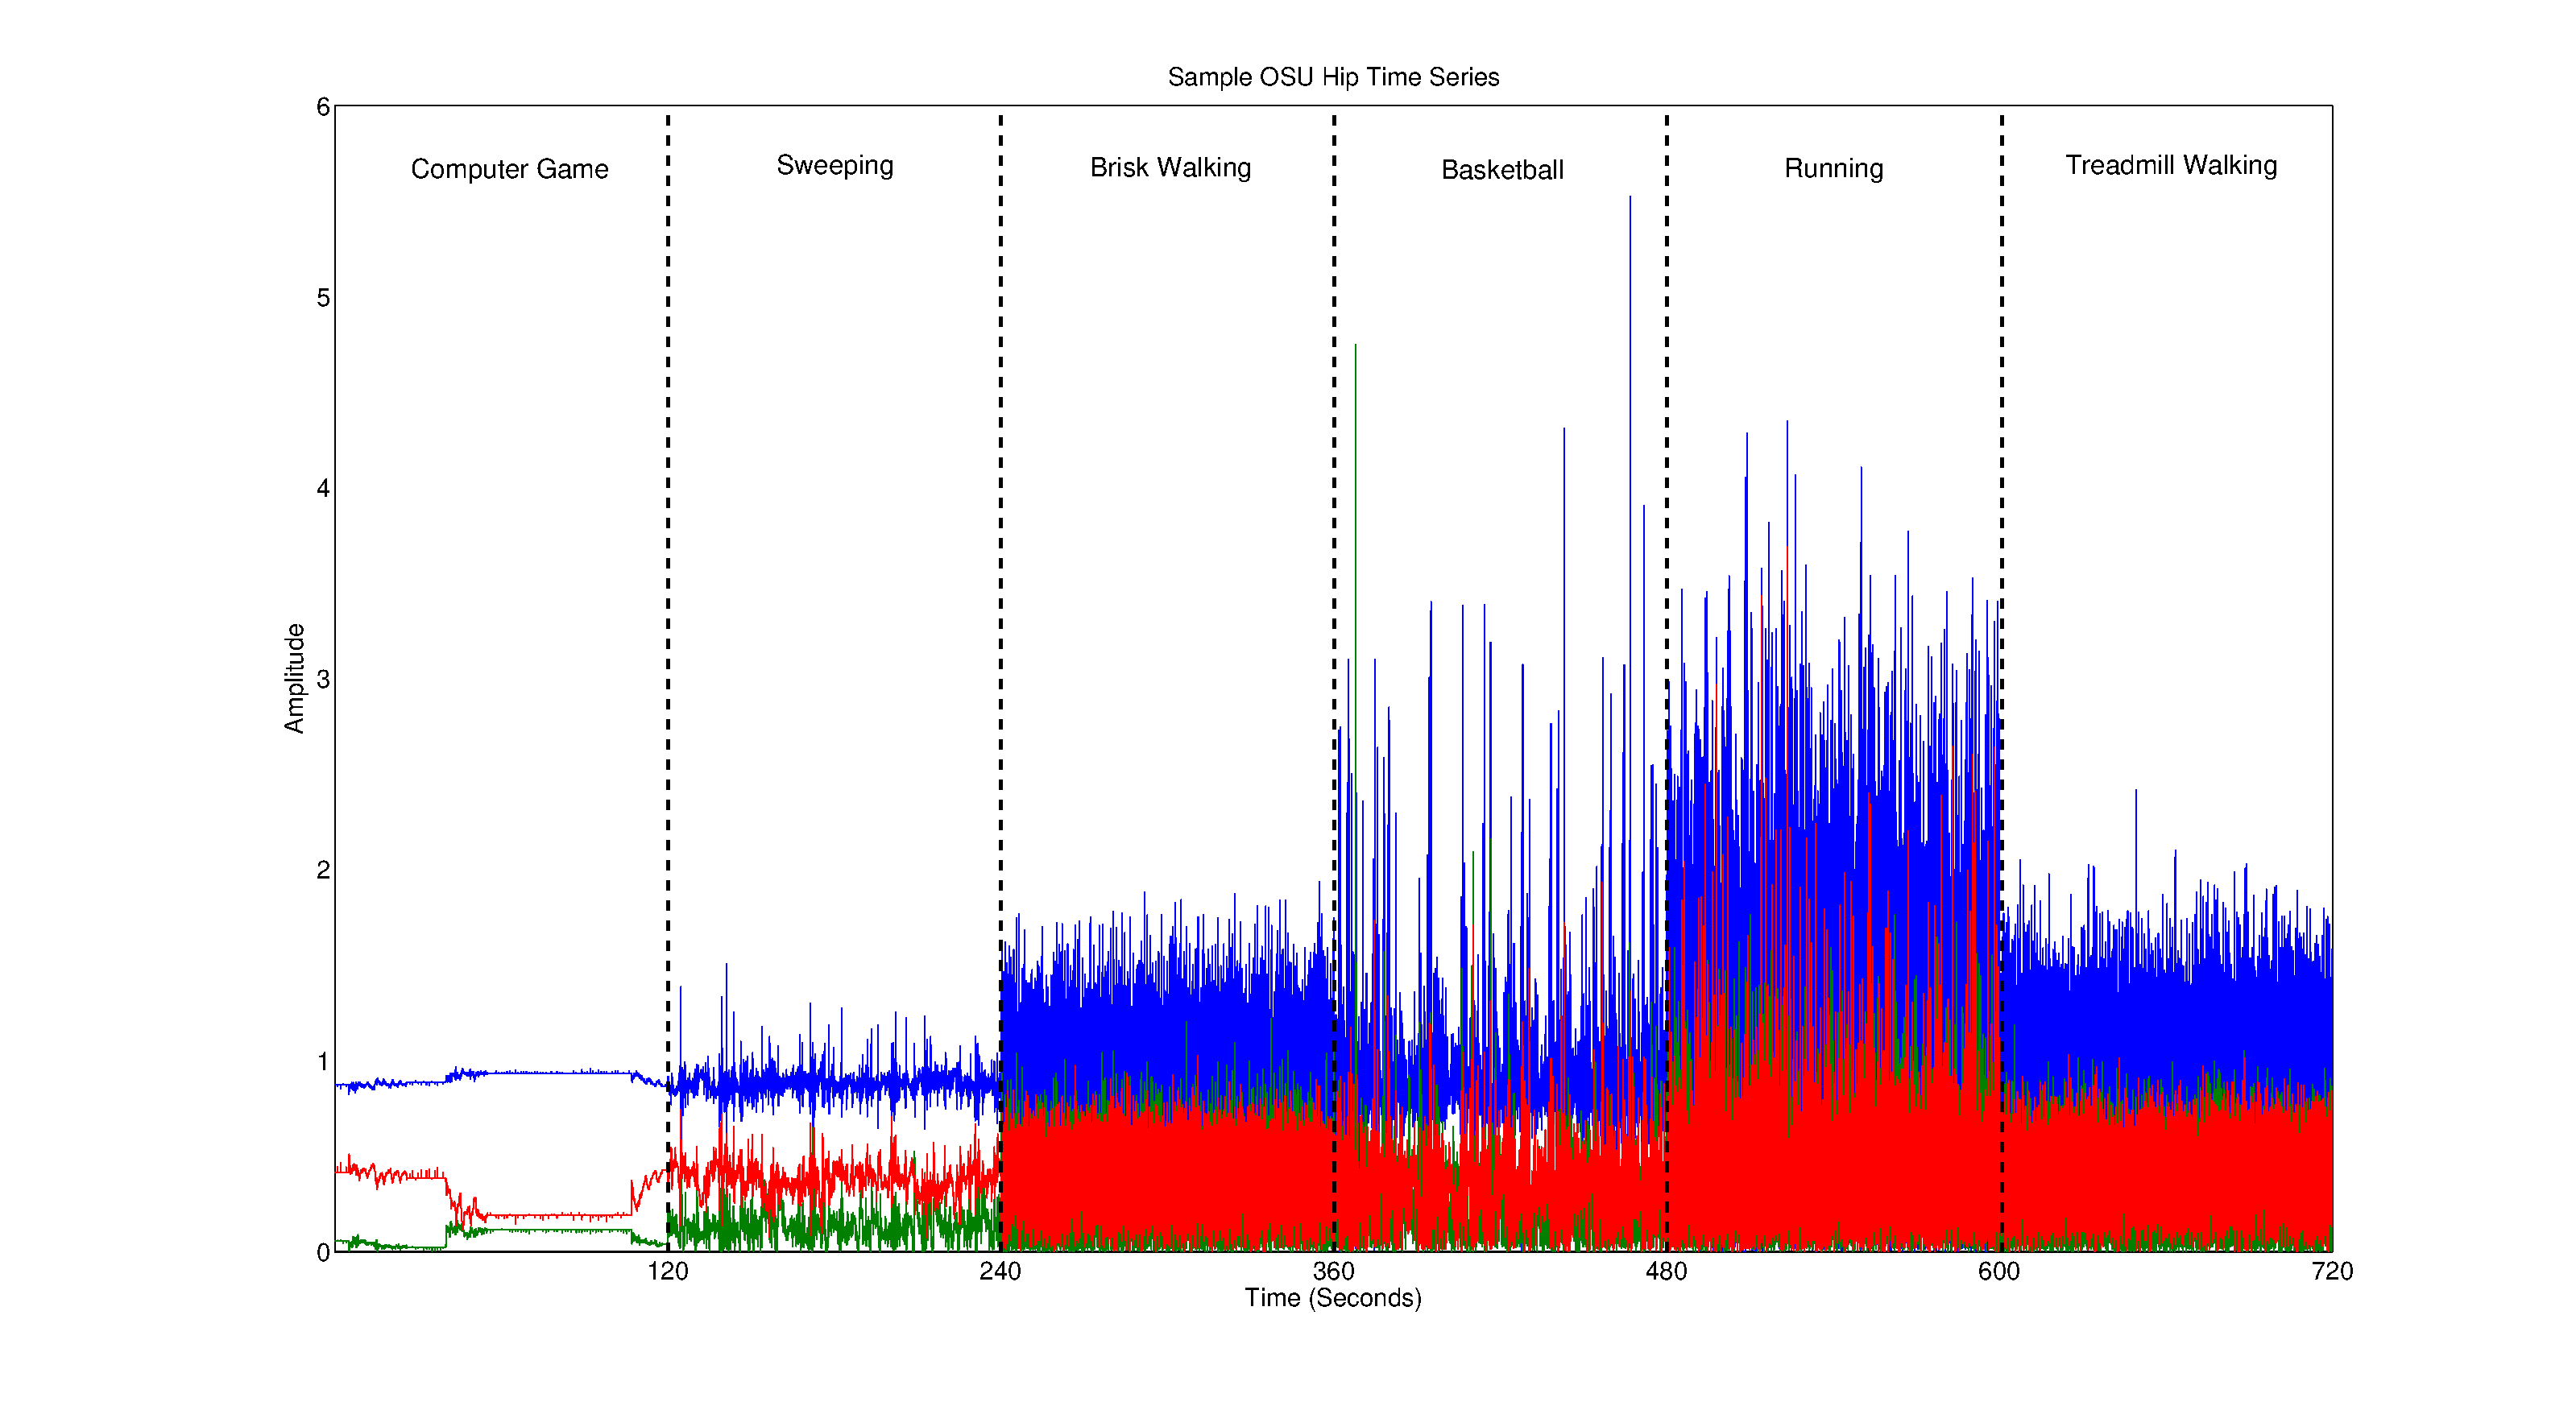
\includegraphics[scale=0.27]{osu_timeseries.pdf}
 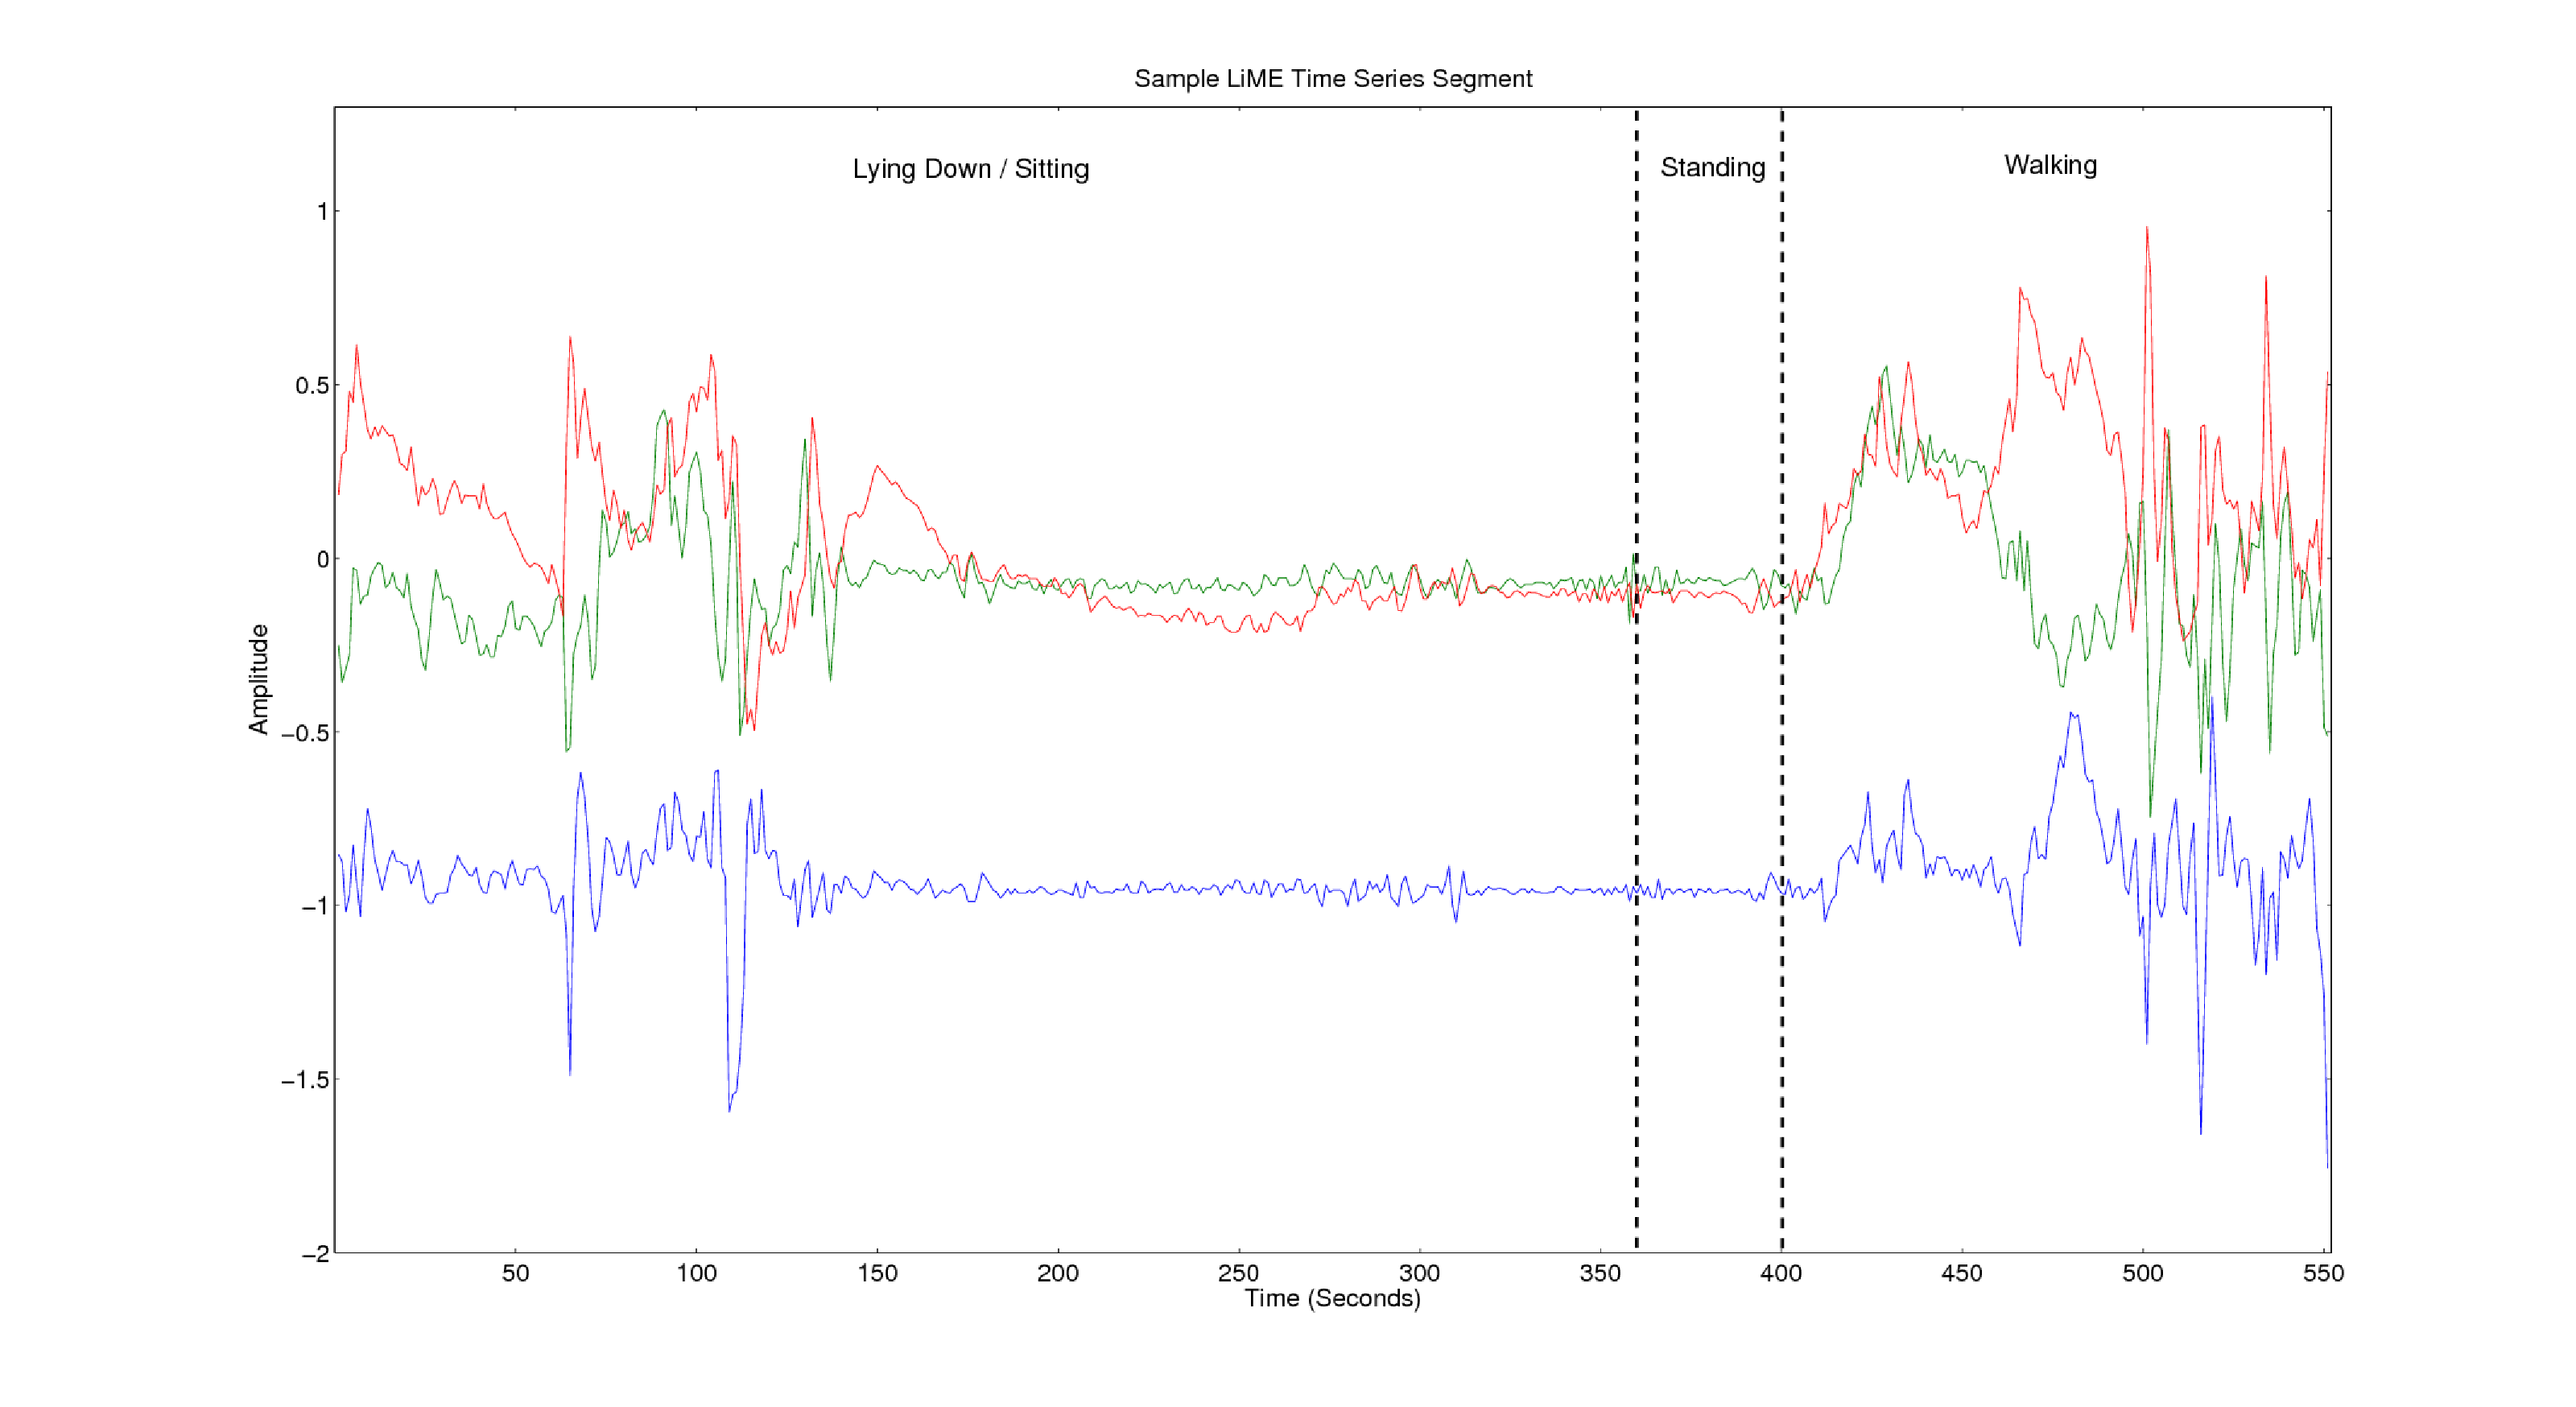
\includegraphics[scale=0.27]{lime_timeseries.pdf}
 \caption{Sample data from the OSU Hip and LiME datasets. Both datasets are
 triaxial and each axis is shown in a different color.}
 \label{fig:timeseries}
\end{figure}

%\begin{figure}
% \centering
% 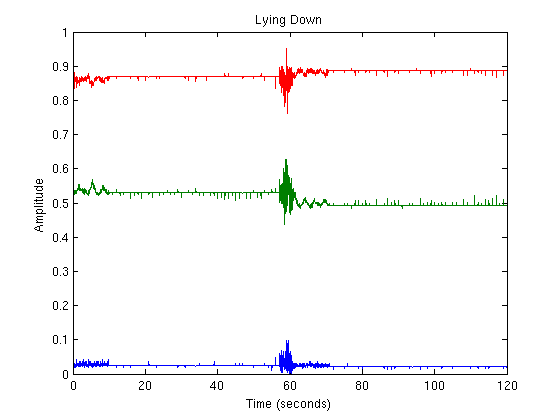
\includegraphics[scale=0.3]{osu_lying.png}
% 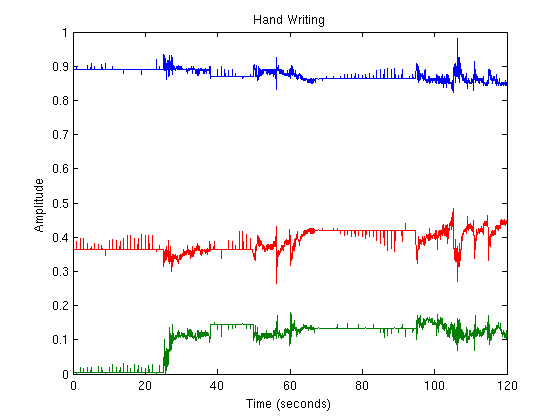
\includegraphics[scale=0.3]{osu_writing.png}
% 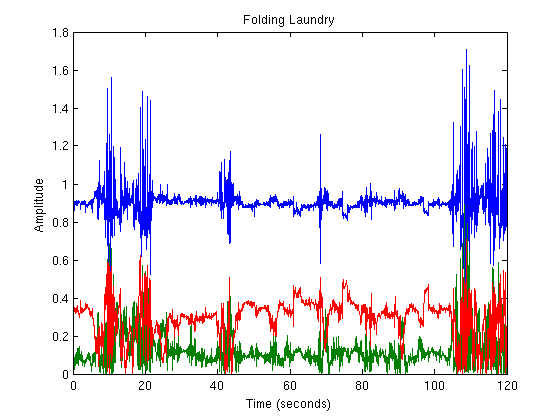
\includegraphics[scale=0.3]{osu_laundry.png}
% 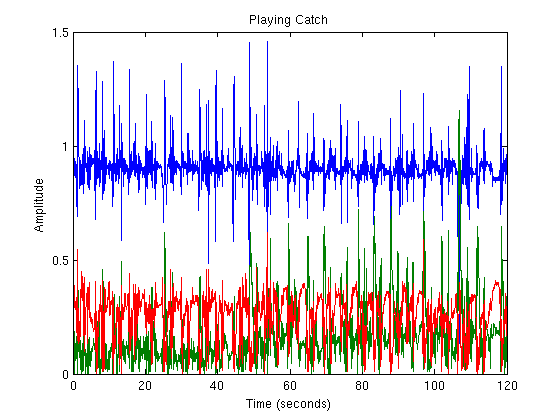
\includegraphics[scale=0.3]{osu_catch.png}
% 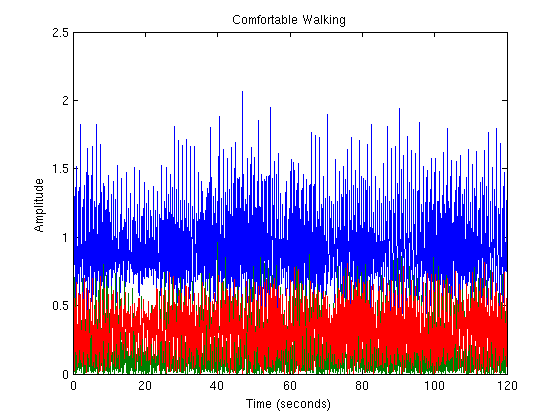
\includegraphics[scale=0.3]{osu_comf_walking.png}
% 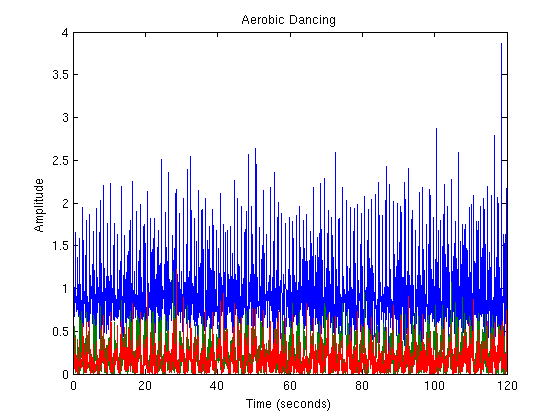
\includegraphics[scale=0.3]{osu_dancing.png}
% 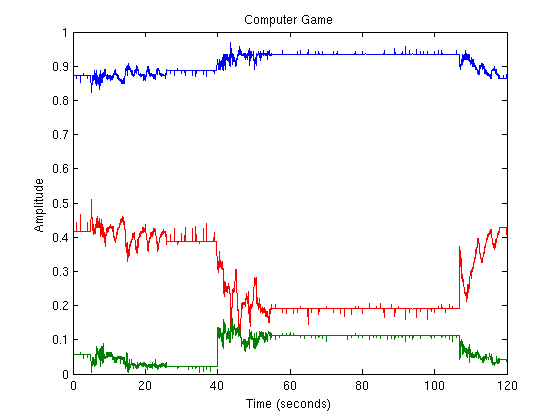
\includegraphics[scale=0.3]{osu_computer.png}
% 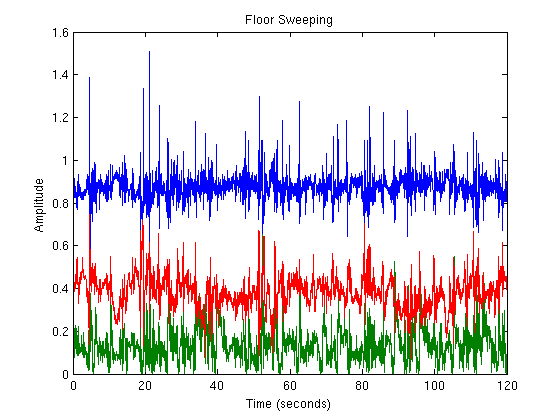
\includegraphics[scale=0.3]{osu_sweeping.png}
% 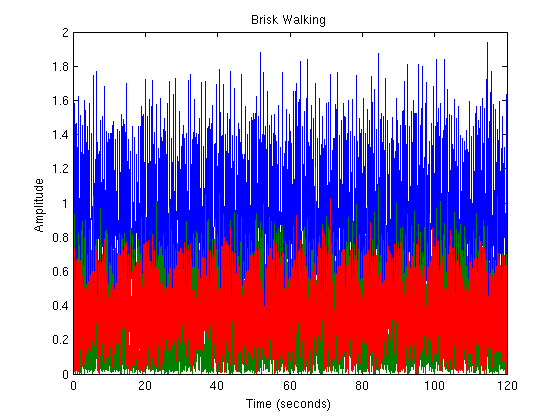
\includegraphics[scale=0.3]{osu_brisk_walking.png}
% 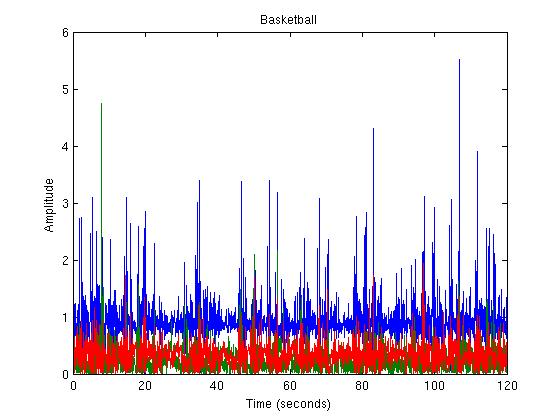
\includegraphics[scale=0.3]{osu_basketball.png}
% 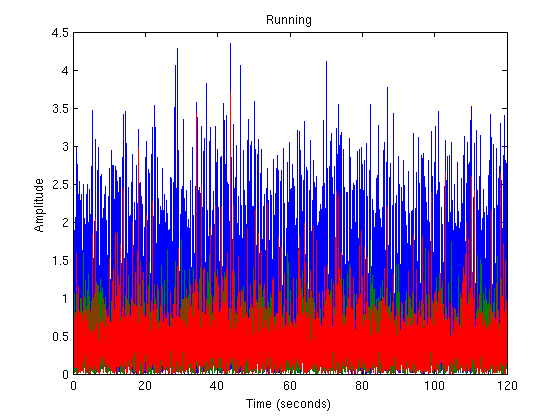
\includegraphics[scale=0.3]{osu_running.png}
% 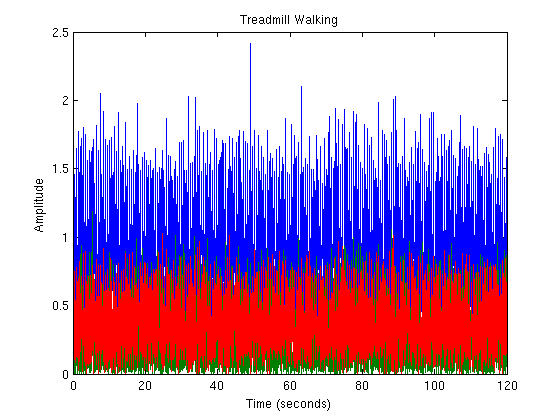
\includegraphics[scale=0.3]{osu_treadmill.png}
% \caption{OSU Hip Activity Samples}
% \label{fig:osu_activities}
%\end{figure}

We determined that several of the activities were very similar and that it would
be difficult to discriminate between them. As a result, we combined some of them together to
create a 7-class version of the data.
The classes were lying down, sitting (hand-writing, computer game),
standing (laundry, sweeping, and catch), walking (comfortable, brisk and treadmill walking),
dancing, running, and basketball.

\subsection{LiME}
This dataset consisted of 23 time series, each containing roughly 10 continuous
days worth of data from an individual subject. It was collected by Helen Brown from
the Univerity of Cambridge, and Gemma Ryde from the University of Stirling, Scotland.
Subjects wore an ActiGraph GT3X+
accelerometer during the entire period, which collected triaxial acceleration data at a frequency
of 30Hz, as well as an activPal inclinometer on their thighs. The inclinometer
provided what we considered the ground truth labels of the data by automatically
delimitting and classifying intervals using the orientation of the subject's thigh at any given moment. It 
classified a horizontal orientation as lying down/sitting,
a vertical orientation as standing, and a combination of the two as walking.
The bottom graph of Figure \ref{fig:timeseries} shows a time series segment
from the dataset that contains all 3 activities.

%\begin{figure}
% \centering
% 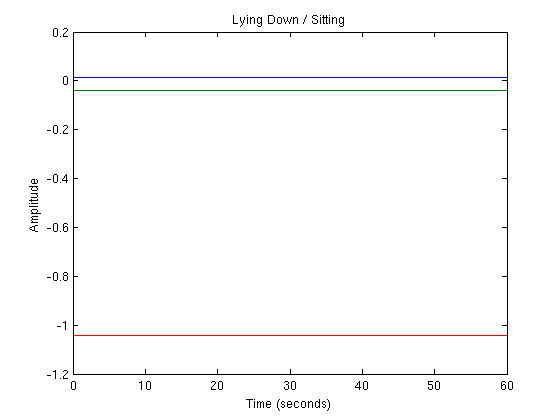
\includegraphics[scale=0.3]{lime_lying.png}
% 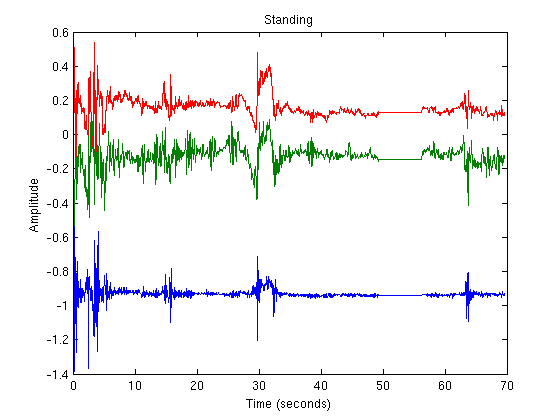
\includegraphics[scale=0.3]{lime_standing.png}
% 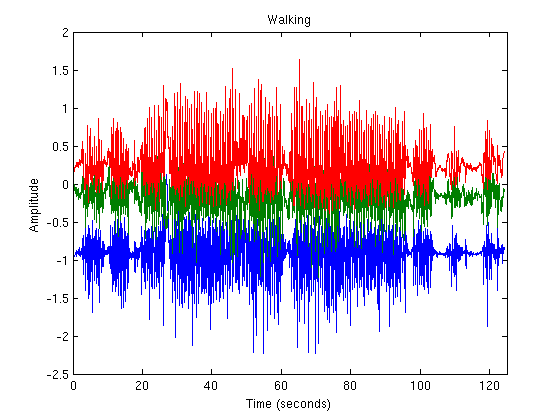
\includegraphics[scale=0.3]{lime_walking.png}
% \caption{LiME Day 1 Activity Samples}
% \label{fig:lime_activities}
%\end{figure}

This dataset was challenging to work with because of its size, as each individual time series
contained roughly 25 million ticks of data. To help alleviate this problem, we split each
time series into individual days. We then treated the first full 24 hour period of data that began at midnight,
from each subject, as one whole dataset (LiME Day 1), and the second such period as a separate dataset
(LiME Day 2). We did not use any data from the remaining days.

In contrast to the OSU Hip dataset, LiME
was not synthetic and activity lengths were variable. For LiME Day 1, the
average activity length was 100 seconds with a standard deviation of 881 seconds, and the
median length was 12 seconds. The average number of activities per time series was
871. As would be expected, statistics for LiME Day 2 were comparable: the
average activity length was 104 seconds with a standard deviation of 803 seconds, and the
median length was 12 seconds. The average number of activities per time series was 834.
The medians were relatively small because many of the activities were short,
while the mean and standard deviations were larger because a few of the
activities were extremely long (e.g. when subjects were sleeping).

\section{Featurization}
To formulate our experiments as classification problems, we split each time series into a set of
non-overlapping windows and represented each window as a feature vector.
How we decided where one window ended (and where the next began) varied between
experiments, and is described in sections \ref{sec:topdown} and \ref{sec:bottomup}. Our feature
set was a large collection of statistics that have been shown to be discriminative
for activity classification in previous research \cite{li09}, \cite{rothney07},
\cite{staudenmeyer09}, \cite{zheng12}. In all we used 18 statistics that were
uniaxial, i.e. were only a function of the data from a single axis of a given window,
as well as one biaxial statistic.
The uniaxial statistics were applied to data from each axis separately, and
the biaxial statistic was applied to data from each of the $C_2^3=3$ possible pairs of
axes, for a total of $18*3+3 = 57$ features.

\vspace{1ex}
\begin{table}[H]
%\small
%\renewcommand{\arraystretch}{1.8}
\centering
\begin{tabular}{|p{15cm}|}  \hline
F1. Sum of values of a period of time: $\sum^T_{i=1} x(i)$.\\ [2ex]
F2. Mean: $\mu_x = \frac{1}{T} \sum^T_{i=1} x(i)$.\\ [2ex]
F3. Standard deviation: $\sigma_x = \sqrt{\frac{1}{T} \sum^T_{i=1} [x(i) - \mu_x]^2}$.\\ [2ex]
F4. Coefficients of variation: $\frac{\sigma_x}{\mu_x}$. \\ [2ex]
F5. Peak-to-peak amplitude: $max \{x(1), ..., x(T)\} - min \{x(1), .., x(T)\}$.\\ [2ex]
F6-10. Percentiles: $10^{th}, 25^{th}, 50^{th}, 75^{th}, 90^{th}$.\\ [2ex]
F11. Interquartile range: difference between the $75^{th}$ and $25^{th}$ percentiles.\\ [2ex]
F12. Lag-one-autocorrelation: $\frac{\sum^{T-1}_{i=1} [x(i) - \mu_x][x(i+1) - \mu_x]}{\sum^T_{i=1} [x(i) - \mu_x]^2}$.\\ [2ex]
F13. Skewness:
 $\frac{\frac{1}{T} \sum^T_{i=1} [x(i) - \mu_x]^3}
{(\frac{1}{T} \sum^T_{i=1} [x(i) - \mu_x]^2)^\frac{3}{2}}$,
 asymmetry of the signal probability distribution.\\ [2ex]
F14. Kurtosis:
 $\frac{\frac{1}{T} \sum^T_{i=1} [x(i) - \mu_x]^4}
{(\frac{1}{T} \sum^T_{i=1} [x(i) - \mu_x]^2)^3} - 3$,
 peakedness of the signal probability distribution.\\ [2ex]
F15. Signal power: $\sum^T_{i=1} x(i)^2$.\\ [2ex]
F16. Log-energy: $\sum^T_{i=1} \log[x(i)^2]$.\\ [2ex]
F17. Peak intensity: number of signal peak appearances.\\ [2ex]
F18. Zero crossings: number of times the signal crosses its median.\\ [2ex]
F19. Correlation between each pair of axes:
 $\frac{\sum^T_{i=1}[x(i)-\mu_x][v(i)-\mu_v]}
{\sqrt{\sum^T_{i=1}[x(i)-\mu_x] \sum^T_{j=1}[v(j)-\mu_v]}}$.\\ [2ex] \hline
\end{tabular}
\caption{Statistics used to convert time series windows into feature vectors
(taken from \cite{zheng13}). $T$ is the number of ticks in the given time
series, $x$ and $v$ are individual axes of the time series data, and $x(i)$
is the $i$th data tick of $x$.}
\end{table}


%Features (from \cite{zheng13})\\ \hline \\ [-1ex]

One discriminative characteristic of an activity is its overall vigorousness.
The sum [F1] and the sample mean [F2] both act as simple and obvious ways
of measuring vigorousness, as more intense activities will tend to involve
higher rates of acceleration during movement. We also used the 10th [F6], 25th [F7],
50th [F8], 75th [F9], and 90th [F10] percentiles of the data, as well as signal
power [F15] and log energy [F16] as supplemental measures of overall activity intensity.

Another characteristic of an activity is how much it varies in intensity. The sample standard
deviation [F3], coefficient of variation [F4], peak-to-peak amplitude [F5],
number of zero crossings [F18], as well as the
interquartile range [F11] were useful for discriminating between activities
with a consistent level of intensity (low variance, etc.) and activities that were more
rhythmic or staccato in intensity (high variance, etc.). 

Lag-one-autocorrelation [F12], skewness [F13], kurtosis [F14], and peak intensity [F17]
were useful for discriminating between
activities that tend to be similar in their overall intensity and variation in intensity,
but that yielded data with other types of difference in shape. Skewness indicates whether the data is
more concentrated above or below its mean. Kurtosis indicates that the data is concentrated
near its mean or conversely that it is fat-tailed. Lag-one-autocorrelation is a measure of
the general relationship between data ticks and their immediate neighbors in time. Peak
intensity is the number of times that the data repeatedly reached its maximum value. 

Finally we looked at a single bimodal statistic across each pair of axes, the correlation
coefficient [F19], which discriminates between activities where acceleration values in one axis
are predictive of acceleration values in another axis, versus activities where that is not the case.

\section{Base Classifiers}

We tested three classification models on the featurized versions of our data:
decision trees, support vector machines, and neural networks. We used R for our
experiments, and used the R libraries `rpart' \cite{rpart}, `e1071' \cite{svm},
and `nnet' \cite{nnet} to build
our decision tree, SVM, and neural network models, respectively. Default rpart values
were used for the decision tree experiments. The rpart package implements a
procedure for automatically tuning how aggressively it prunes its decision tree
models, and hence our validation set was not used to tune this parameter. 
For the neural net experiments, 
the maximum number of iterations was set to 100000, and the maximum number of
weights was set to 1000000.

For the OSU Hip experiments we tuned the
cost parameter $C$ of the svm on the validation set with 6 values:
$\{0.01,0.1,1,10,100,1000\}$. The single-layer feed-forward neural network took
two tuning parameters, and we tuned with each 2-tuple from the set $N \times W$,
where $N = \{1,2, \ldots, 30\}$ was the numbers of nodes in the hidden layer, and 
$W = \{0,0.5,1\}$ was the weight decay parameter.

Since the LiME datasets were an order of magnitude larger, we tuned them
slightly differently because of time constraints. Setting the $C$ parameter to
1000 proved to be very computationally expensive for the SVM model; instead we tuned $C$
from the values $\{0.01,0.1,1,10,100\}$. Running $30*3=90$ tuning experiments
for the neural networks was also prohibitively expensive; instead we tuned using
values from $N \times W = \{5,10,15\} \times \{0,0.5,1\}$.

\section{Top-Down Approach}
\label{sec:topdown}

\subsection{Change Point Detection}
For this approach, the data was split into non-overlapping segments for
featurization using techniques from the statistical field of change point detection.
Change point detection has found application in many problem domains that require analysis of time series data
from dynamic systems, including failure detection \cite{bae13}, quick detection of
attacks on computer networks \cite{tartakovsky06}, and monitoring of heartbeat fluctuations during
sleep \cite{staudacher05}. Change point detection assumes that each tick of a time series is a draw from some
process, but that the process may suddenly change as time passes.
The goal is to predict when these changes have occurred.
A \emph{score} is generated for each time tick, and if the score is
above a given threshold a change is predicted to have occurred between that tick
and its immediate predecessor. To generate a score at
a time tick, a window of data that immediately preceeds it (the
\emph{reference data}) is compared to it along with a window of data that immediately follows it
(the \emph{test data}).

\begin{figure}
 \centering
 \includegraphics[scale=0.8]{cpd_ref_test_new.png}
 \caption{Change Point Detection}
 \label{fig:cpd_ref_test.png}
\end{figure}

Model-based approaches to change point detection assume that each tick in
a time series is a draw from some underlying probability distribution.
Scores are generated by estimating the distribution of the reference data
and the test data, and then by calculating the likelihood
that the two distributions are different.
Where it is reasonable to assume that the data belongs to a particular
family of distributions then parametric estimation methods have been employed
\cite{thatte11}. If no such modeling assumptions are reasonable then 
non-parametric methods have also been found to be viable \cite{matteson12}.
Distance-based approaches such as Singular Spectrum Analysis
generate scores through other metrics of 
dissimilarity or difference between the reference data and the test data
\cite{moskvina03}.
Notationally, we say that for each tick $i$ in a time series:

\[
s_i = D(x_{r,i}, x_{t,i})
\]

Where $s_i$ is the score of the $i$th tick, $x_{r,i}$ is the reference
data associated with the $i$th tick, $x_{t,i}$ is the test data
associated with the $i$th tick, and $D(A,B)$ is a function that computes the
dissimiliarity between a matrix of data $A$ and matrix of data $B$, and varies
between change point algorithms. Note that for a given
algorithm it may not be possible to generate scores right at the very beginning
of the time series (insufficient reference data) or at the very end of a time
series (insufficient test data).

\subsection{Experimental Setup}

There are many different modeling assumptions and associated algorithms
for generating change point detection scores, and one simple baseline approach that we 
wanted to test was the Shewhart Control Chart. This approach assumes that the reference data is drawn from a
multivariate normal distribution, and that scores are calculated by the Mahalanobis
distance of the target time tick from the estimated multivariate normal:

\[
s_i = \sqrt{(\bar{x}_{r,i} - x_i)^T \, S_{r,i}^{-1} \, (\bar{x}_{r,i} - x_i)}
\]

where $\bar{x}_{r,i}$ is the sample mean of the reference data, $S_{r,i}$
is the sample covariance matrix of the reference data, and $x_i=x_{t,i}$ is
the $i$th data point \cite{shewhart26}.

We were also interested in testing the performance of a newer and more
sophisticated change point detection algorithm: the
Kullback-Leibler Importance Estimation Procedure (KLIEP),
introduced by Kawahara and Sugiyama \cite{sugiyama09} \cite{sugiyama08}.
This approach generates scores using the Kullback-Leibler (KL)
divergence between the reference data and the test data. One method of doing this
is to estimate the density of the reference distribution and test distribution
separately, and then compare them using a likelihood ratio
(known in the change point detection literature as \emph{importance}). 
Instead, KLIEP estimates the importance directly using a non-parametric model.

Let the estimate of the importance $\hat{R}$ be represented by this model:

\[
\hat{R} = \frac{p_{t}}{\hat{p}_{r}} = \sum_{j=1}^{n_{t}} \alpha_j K_G(x,x_{t,j})
\]

Where $p_{r}$ and $p_{t}$ are the probability densities of the reference data and the test
data, $n_{t}$ is the number of ticks in the test window, $\alpha$ is a
vector of model parameters to solve for, $x$ is the concatenation of the reference and the
test data, $x_{t,j}$ is the $j$th element of the test data,
and $K_G(A,B)$ is the Gaussian kernel with width $\sigma$:

\[
K_G(A,B) = \exp \left(-\frac{||A-B||^2}{2\sigma^2}\right)
\]

Now solve for $\alpha$ so that the empirical KL divergence between $\hat{p}_{t}$ and
$p_{t} = p_{r}\hat{R}$ is minimized, which is equivalent to the following convex optimization
problem:

\[
\begin{dcases}
 \max_{\alpha} \quad \sum_{j=1}^{n_t} \, \log \left( \sum_{k=1}^{n_t} \alpha_k K_G(x_{t,j}, x_{t,k}) \right) \\
 \,\, \text{s.t.} \quad\, \frac{1}{n_r} \sum_{j=1}^{n_r} \sum_{k=1}^{n_t} \alpha_k K_G(x_{r,j},x_{t,k}) = 1 \\
 \qquad \quad \text{and} \; \alpha_1 \ldots \alpha_{n_t} \ge 1
\end{dcases}
\]

Finally, the scores that we wish to generate are just the estimate of the importance given by the
solution to the complex optimization problem, i.e. $s_i = \hat{R}_i$.

Since this approach uses a Gaussian kernel, it requires the selection of
a kernel width $\sigma$ for each time tick. We used an implementation of
KLIEP that is available at Sugiyama's website, which included a cross-validation
procedure for the value of $\sigma$. The CV procedure chooses a number of disjoint
splits of the test data along with a number of different candidate $\sigma$'s, and runs
KLIEP with each combination of split and candidate $\sigma$. Then it chooses the candidate $\sigma$
that, on the average across all of the splits, maximizes the KL divergence (the
$\max_{\alpha}$ equation above) the most.

For the OSU Hip dataset, we used this CV procedure io choose the the kernel width at each individual time tick. This computationally
intensive approach was impractical for the UQ dataset because it is orders of magnitude larger,
so instead of running it on every tick of that data, we ran the CV procedure on a number of
random ticks drawn from the data. From this we were able
to empirically identify 0.01 as a plausible $\sigma$, and so fixed $\sigma$
at that value for our experiments on that dataset.

Previous research \cite{zheng12} found that on the average a window size of 10
seconds contained just enough information to discriminate well between OSU Hip activities.
Since this window size worked well in previous experiments, and since the 
activities of the UQ dataset were comparable in average length, we decided to
fix our reference window size at 10 seconds for both datasets. Because we were interested in
minimizing detection time, and because 1 second was the smallest window that
we felt could provide some information about an activity, we fixed our test
window size at 1 second for both datasets.

Once scores were generated, we tested a number of threshold values that determined which
scores were high enough to be considered a predicted change-point.
Threshold values were chosen by considering the false positive rates of
change prediction for the change point detection algorithms. A smaller false positive rate
corresponded to a higher and more conservative threshold, which split the
time series into fewer segments for featurization. A larger false positive rate
corresponded to a lower threshold, which split the time series into more segments.

\section{Bottom-Up Approach}
\label{sec:bottomup}

\subsection{HMMs}

Once we had created our methodology for splitting up time series using change-
point detection, we decided to test it against a more standard,
baseline technique. For this approach, we used the Hidden Markov Model to take
advantage of the sequential nature of our data. An HMM is a temporal graphical model
that contains a set of hidden states $H = \{H_0,H_1, \ldots, H_w\}$ as well as a set of
observed states $O = \{O_1,O_2, \ldots, O_w\}$ (Figure \ref{fig:hmm}). An index
of either type of state represents a point in time, such that if there exists
two indices $i$ and $j$ where $i < j$, $i$ is thought of as having happened
before $j$. Each hidden state in the model has one of a discrete set of values associated
with it drawn from $X=\{X_1,X_2, \ldots, X_{\ell}\}$, and each observed state has one
of a discrete set of values associated with it drawn from $Y=\{Y_1,Y_2, \ldots, Y_m\}$.
The values of the hidden states are unknown, and the values of the observable
states are known.
It is also assumed that, as indicated by Figure \ref{fig:hmm}, the
value of an observable state $O_i$ is dependent on the corresponding
hidden state $H_i$, and that the value of any hidden state $H_i$ is dependent only on
its immediate predecessor $H_{i-1}$.

Furthermore, the dependencies between hidden states and their followers are
assumed to be described by a stationary stochastic process known as the
\emph{transition model}, \mbox{$T: X^2 \rightarrow [0,1]$}. The dependencies
between a hidden state and its adjacent observable state are assumed to be part
of a separate but also stationary stochastic process known as the
\emph{observation model}, $S: X \times Y \rightarrow [0,1]$. In other words, both
models can be thought of as a function of two values, that output the
probability of a change from the first value to the second via a dependency
arc in the HMM. The usual approach to estimating $T$ and $S$ given only
$O$ is a flavor of expectation maximation known as the Baum-Welch algorithm,
which is useful for finding $\hat{T}$ and $\hat{S}$ that are locally maximally
likely. However, suppose a \emph{training HMM} $\langle H_{tr},O_{tr} \rangle$
with the same model parameters is given, and the values of all of its hidden states as well as its
observable states are known. $T$ and $S$ are then approximated by the
following global maximum likelihood estimators:

\[
\hat{T}(X_i,X_j) = \frac{|\{H_k \in H_{tr} \; | \; H_k=X_i \; \text{and} \; H_{k+1}=X_j\}|} {|\{H_k \in H_{tr} \; | \; H_k=X_i\}|}
\]

\[
\hat{S}(X_i,Y_j) = \frac{|\{H_k \in H \; | \; H_k=X_i \; \text{and} \; O_k=Y_j\}|} {|\{H_k \in H \; | \; H_k=X_i\}|}
\]

\begin{figure}
 \centering
 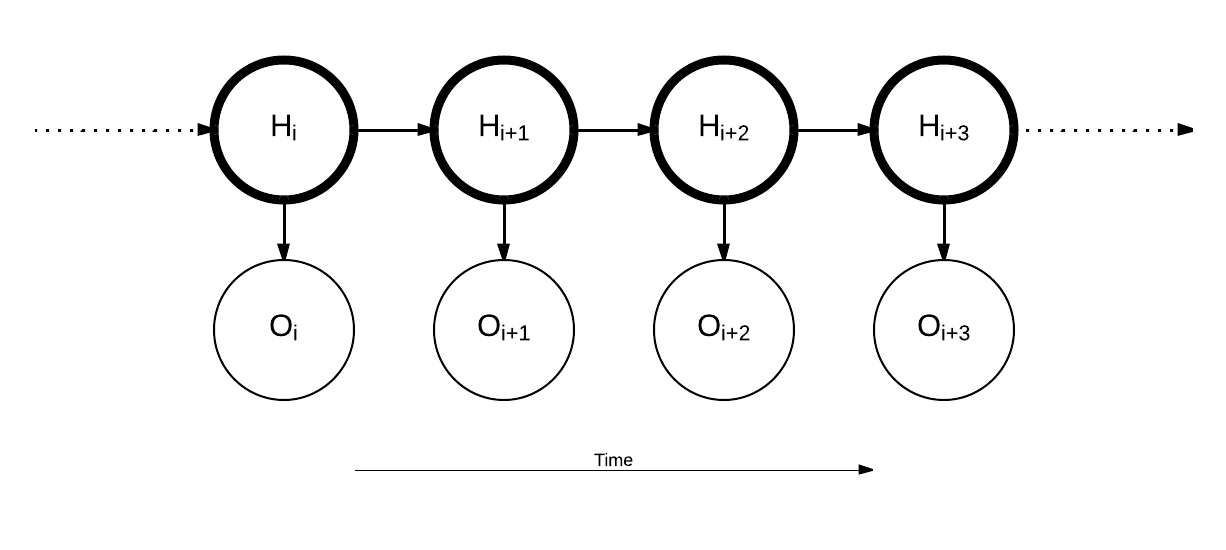
\includegraphics[scale=0.3]{hmm.png}
 \caption{Visual Interpretation of an HMM}
 \label{fig:hmm}
\end{figure}

Finally, if all of the values of $O$ are known, and we are given
a $\hat{T}$ and an $\hat{S}$ estimated from a training HMM, then the goal we are interested in
is to use that information (along with the model assumptions)
to find the most likely values for each state in $H$. There
exists a polynomial-time dynamic programming solution to this problem known as
the Viterbi algorithm. \cite{russell10}

\subsection{Experimental Setup}

For our experiments we began by splitting each time series into small non-overlapping windows. Within a
given experiment the window size was fixed, but across different experiments we
tested window sizes of length $\{1,2, \ldots ,20\}$. Once the time series were
split they were featurized. Classification
models were built with training data,
and tuned (in the case of the svm and neural net models) using validation data,
in the same way that has already been described previously in this chapter.

Unlike the change-point detection experiments, this experiment required
that the data be split into 4 equal parts: training (classifier), validation,
training (HMM), and testing) rather than 3. 
Here we formulated the problem of making predictions on the testing set in terms
of an HMM, first by treating the second training set as a training HMM. Each
window of the second training set was treated as a time index ${1,2, \ldots, n}$.
In our datasets we
let $H$ be the ground truth activity classes of the windows, and $O$ be the
predicted activity classes of the windows. We used the precedure above to
calculate $\hat{T}$ and $\hat{S}$, and assumed that these estimates held for
the testing set as well as the second training set. We then used the
tuned base classifier to predict on the testing set, giving us $O$. Finally,
we used $O$, $\hat{T}$, and $\hat{S}$ to run the Viterbi algorithm on the
testing set and predict the ground truth activity classes $H$.


\section{Performance Metrics}
\begin{figure}[h]
 \centering
 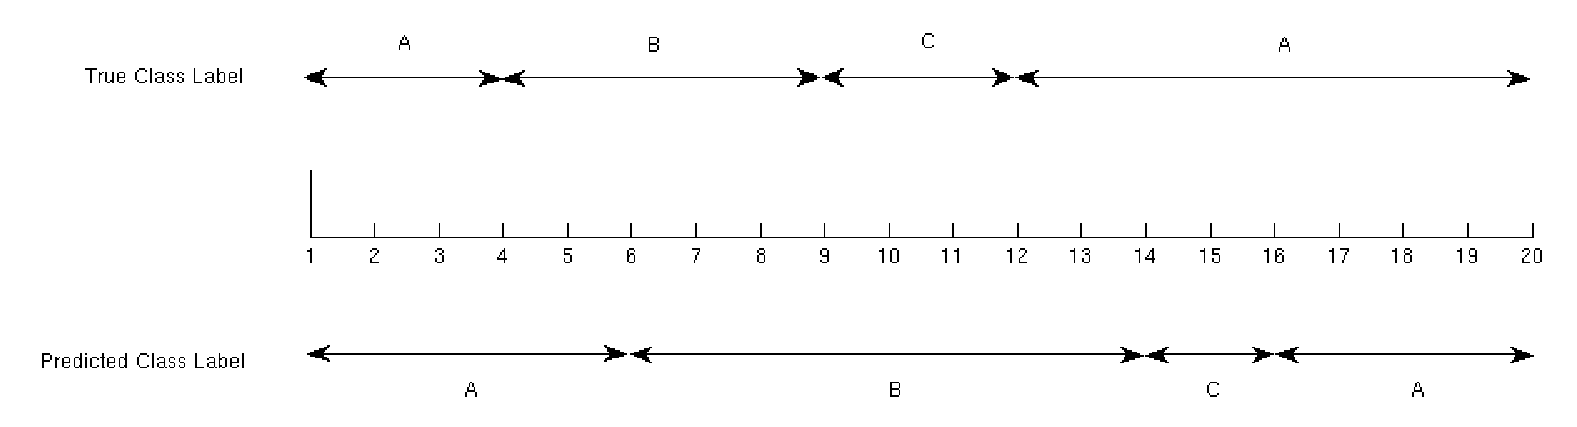
\includegraphics[scale=0.45]{performance.pdf}
 \caption{An example time series with 20 ticks of data, from a dataset with
  three classes: A, B, and C. Four true class labels and their associated
  windows are shown above the axis; four predicted class
  labels and their associated windows are shown below the axis.}
 \label{fig:performance}
\end{figure}

To measure the performance of our classification algorithms we used
two metrics. Accuracy is defined as the number of ticks that an algorithm
correctly classifies in a time series, over the total number of ticks
in the time series. Accuracy is computed by counting the number of
correctly predicted ticks for each true window separately, summing the counts,
and dividing by the total number of ticks. An example section of a time series
is shown in Figure \ref{fig:performance}, and the accuracy of the shown
predictions is given as follows:

\[
\text{Accuracy} = \frac{\text{CPT(A}_1) + \text{CPT(B)} + \text{CPT(C)} + \text{CPT(A}_2)}{(\text{Total number of ticks})} =
\]

\[
\frac{3 + 3 + 0 + 4}{20} = 50\%
\]

where CPT(.) is the number of correctly predicted ticks in an interval, and
A$_1$ and A$_2$ are the true class "A" windows.

Since we were also interested in our algorithms'
feasibility for activity classification in real time, we used detection time as
a second metric. Detection time is computed by counting how many ticks are
required for a prediction algorithm to start correctly predicting the class,
after a true window begins. These counts are summed, and then divided by the number of
true activities.

Consider again the time series segment in Figure \ref{fig:performance}.
Over the true window beginning at tick 1 (class A), the algorithm predicts A
immediately, so the detection time for that window is 0. Over the second true
window beginning at tick 4 (class B), the algorithm does not start predicting
B until tick 6 so the detection time for that window is $6-4=2$. Over the third
true window starting at tick 9 (class C),
the algorithm never predicts C, so the detection time for that window is 3, the
full length of the window. Over the fourth true window starting at tick 12 (class A), the
algorithm starts to predict C at tick 14, but does not predict A until tick 16,
so the detection time for that window is $16 - 12 = 4$. Thus the average
detection time over the time series segment is:

\[
\frac{(0 + 2 + 3 + 4) \; \text{ticks}}{4 \; \text{windows}} = \frac{9}{4} \; \text{ticks per window}
\]

In the change-point detection experiments accuracy and detection time were
averaged over 30 random splits of the given dataset into training, validation, and
testing sets. Because the HMM experiments were more computationally
expensive, accuracy and detection time were averaged over 10 random splits of
the given dataset into training (base classifier), validation, training (HMM),
and testing sets.
